\documentclass[]{article}
\usepackage{lmodern}
\usepackage{amssymb,amsmath}
\usepackage{ifxetex,ifluatex}
\usepackage{fixltx2e} % provides \textsubscript
\ifnum 0\ifxetex 1\fi\ifluatex 1\fi=0 % if pdftex
  \usepackage[T1]{fontenc}
  \usepackage[utf8]{inputenc}
\else % if luatex or xelatex
  \ifxetex
    \usepackage{mathspec}
  \else
    \usepackage{fontspec}
  \fi
  \defaultfontfeatures{Ligatures=TeX,Scale=MatchLowercase}
\fi
% use upquote if available, for straight quotes in verbatim environments
\IfFileExists{upquote.sty}{\usepackage{upquote}}{}
% use microtype if available
\IfFileExists{microtype.sty}{%
\usepackage{microtype}
\UseMicrotypeSet[protrusion]{basicmath} % disable protrusion for tt fonts
}{}
\usepackage[margin=1in]{geometry}
\usepackage{hyperref}
\PassOptionsToPackage{usenames,dvipsnames}{color} % color is loaded by hyperref
\hypersetup{unicode=true,
            pdftitle={Standard Errors in OLS},
            pdfauthor={Luke Sonnet},
            colorlinks=true,
            linkcolor=Maroon,
            citecolor=Blue,
            urlcolor=blue,
            breaklinks=true}
\urlstyle{same}  % don't use monospace font for urls
\usepackage{color}
\usepackage{fancyvrb}
\newcommand{\VerbBar}{|}
\newcommand{\VERB}{\Verb[commandchars=\\\{\}]}
\DefineVerbatimEnvironment{Highlighting}{Verbatim}{commandchars=\\\{\}}
% Add ',fontsize=\small' for more characters per line
\usepackage{framed}
\definecolor{shadecolor}{RGB}{248,248,248}
\newenvironment{Shaded}{\begin{snugshade}}{\end{snugshade}}
\newcommand{\AlertTok}[1]{\textcolor[rgb]{0.94,0.16,0.16}{#1}}
\newcommand{\AnnotationTok}[1]{\textcolor[rgb]{0.56,0.35,0.01}{\textbf{\textit{#1}}}}
\newcommand{\AttributeTok}[1]{\textcolor[rgb]{0.77,0.63,0.00}{#1}}
\newcommand{\BaseNTok}[1]{\textcolor[rgb]{0.00,0.00,0.81}{#1}}
\newcommand{\BuiltInTok}[1]{#1}
\newcommand{\CharTok}[1]{\textcolor[rgb]{0.31,0.60,0.02}{#1}}
\newcommand{\CommentTok}[1]{\textcolor[rgb]{0.56,0.35,0.01}{\textit{#1}}}
\newcommand{\CommentVarTok}[1]{\textcolor[rgb]{0.56,0.35,0.01}{\textbf{\textit{#1}}}}
\newcommand{\ConstantTok}[1]{\textcolor[rgb]{0.00,0.00,0.00}{#1}}
\newcommand{\ControlFlowTok}[1]{\textcolor[rgb]{0.13,0.29,0.53}{\textbf{#1}}}
\newcommand{\DataTypeTok}[1]{\textcolor[rgb]{0.13,0.29,0.53}{#1}}
\newcommand{\DecValTok}[1]{\textcolor[rgb]{0.00,0.00,0.81}{#1}}
\newcommand{\DocumentationTok}[1]{\textcolor[rgb]{0.56,0.35,0.01}{\textbf{\textit{#1}}}}
\newcommand{\ErrorTok}[1]{\textcolor[rgb]{0.64,0.00,0.00}{\textbf{#1}}}
\newcommand{\ExtensionTok}[1]{#1}
\newcommand{\FloatTok}[1]{\textcolor[rgb]{0.00,0.00,0.81}{#1}}
\newcommand{\FunctionTok}[1]{\textcolor[rgb]{0.00,0.00,0.00}{#1}}
\newcommand{\ImportTok}[1]{#1}
\newcommand{\InformationTok}[1]{\textcolor[rgb]{0.56,0.35,0.01}{\textbf{\textit{#1}}}}
\newcommand{\KeywordTok}[1]{\textcolor[rgb]{0.13,0.29,0.53}{\textbf{#1}}}
\newcommand{\NormalTok}[1]{#1}
\newcommand{\OperatorTok}[1]{\textcolor[rgb]{0.81,0.36,0.00}{\textbf{#1}}}
\newcommand{\OtherTok}[1]{\textcolor[rgb]{0.56,0.35,0.01}{#1}}
\newcommand{\PreprocessorTok}[1]{\textcolor[rgb]{0.56,0.35,0.01}{\textit{#1}}}
\newcommand{\RegionMarkerTok}[1]{#1}
\newcommand{\SpecialCharTok}[1]{\textcolor[rgb]{0.00,0.00,0.00}{#1}}
\newcommand{\SpecialStringTok}[1]{\textcolor[rgb]{0.31,0.60,0.02}{#1}}
\newcommand{\StringTok}[1]{\textcolor[rgb]{0.31,0.60,0.02}{#1}}
\newcommand{\VariableTok}[1]{\textcolor[rgb]{0.00,0.00,0.00}{#1}}
\newcommand{\VerbatimStringTok}[1]{\textcolor[rgb]{0.31,0.60,0.02}{#1}}
\newcommand{\WarningTok}[1]{\textcolor[rgb]{0.56,0.35,0.01}{\textbf{\textit{#1}}}}
\usepackage{graphicx,grffile}
\makeatletter
\def\maxwidth{\ifdim\Gin@nat@width>\linewidth\linewidth\else\Gin@nat@width\fi}
\def\maxheight{\ifdim\Gin@nat@height>\textheight\textheight\else\Gin@nat@height\fi}
\makeatother
% Scale images if necessary, so that they will not overflow the page
% margins by default, and it is still possible to overwrite the defaults
% using explicit options in \includegraphics[width, height, ...]{}
\setkeys{Gin}{width=\maxwidth,height=\maxheight,keepaspectratio}
\IfFileExists{parskip.sty}{%
\usepackage{parskip}
}{% else
\setlength{\parindent}{0pt}
\setlength{\parskip}{6pt plus 2pt minus 1pt}
}
\setlength{\emergencystretch}{3em}  % prevent overfull lines
\providecommand{\tightlist}{%
  \setlength{\itemsep}{0pt}\setlength{\parskip}{0pt}}
\setcounter{secnumdepth}{0}
% Redefines (sub)paragraphs to behave more like sections
\ifx\paragraph\undefined\else
\let\oldparagraph\paragraph
\renewcommand{\paragraph}[1]{\oldparagraph{#1}\mbox{}}
\fi
\ifx\subparagraph\undefined\else
\let\oldsubparagraph\subparagraph
\renewcommand{\subparagraph}[1]{\oldsubparagraph{#1}\mbox{}}
\fi

%%% Use protect on footnotes to avoid problems with footnotes in titles
\let\rmarkdownfootnote\footnote%
\def\footnote{\protect\rmarkdownfootnote}

%%% Change title format to be more compact
\usepackage{titling}

% Create subtitle command for use in maketitle
\newcommand{\subtitle}[1]{
  \posttitle{
    \begin{center}\large#1\end{center}
    }
}

\setlength{\droptitle}{-2em}

  \title{Standard Errors in OLS}
    \pretitle{\vspace{\droptitle}\centering\huge}
  \posttitle{\par}
    \author{Luke Sonnet}
    \preauthor{\centering\large\emph}
  \postauthor{\par}
    \date{}
    \predate{}\postdate{}
  
\usepackage{bm}

\begin{document}
\maketitle

{
\hypersetup{linkcolor=black}
\setcounter{tocdepth}{1}
\tableofcontents
}
\newcommand{\y}{\mathbf{y}}
\newcommand{\X}{\mathbf{X}}
\newcommand{\bepsilon}{\bm{\epsilon}}
\newcommand{\bbeta}{\bm{\beta}}
\newcommand{\E}{\mathbb{E}}
\newcommand{\V}{\mathbb{V}}

This document reviews common approaches to thinking about and estimating
uncertainty of coefficients estimated via OLS. Much of the document is
taken directly from
\href{https://web.stanford.edu/~mrosenfe/soc_meth_proj3/matrix_OLS_NYU_notes.pdf}{these
very clear notes}, Greene's Econometric Analysis, and slides by Chad
Hazlett. This document was originally designed for first-year students
in the UCLA Political Science statistics sequence.

\hypertarget{variance-covariance-of-hatbmbeta}{%
\section{\texorpdfstring{Variance-Covariance of
\(\hat{\bm{\beta}}\)}{Variance-Covariance of \textbackslash hat\{\textbackslash bm\{\textbackslash beta\}\}}}\label{variance-covariance-of-hatbmbeta}}

Take the classic regression equation
\[\mathbf{y}= \mathbf{X}\bm{\beta}+ \bm{\epsilon}\] where \(\mathbf{y}\)
is an \(n\times 1\) outcome vector, \(\mathbf{X}\) is an \(n \times p\)
matrix of covariates, \(\bm{\beta}\) is an \(n \times 1\) vector of
coefficients, and \(\bm{\epsilon}\) is an \(n \times 1\) vector of
noise, or errors. Using OLS, our estimate of \(\bm{\beta}\) is
\[\hat{\bm{\beta}} = (\mathbf{X}^\top \mathbf{X})^{-1} \mathbf{X}^\top \mathbf{y}\]

This is just an estimate of the coefficients. We also would like to
understand the variance of this estimate to quantify our uncertainty and
possibly to perform significance tests. We can derive an explicit
function that represents the variance of our estimates,
\(\mathbb{V}[\hat{\bm{\beta}}|\mathbf{X}]\), given that \(\mathbf{X}\)
is fixed.

What we are interested in is
\(\mathbb{V}[\hat{\bm{\beta}}|\mathbf{X}]\), which is the variance of
all the estimated coefficients \(\hat{\bm{\beta}}\) and the covariance
between our coefficients. We can represent this as

\[
\mathbb{V}[\hat{\bm{\beta}}|\mathbf{X}] = 
\begin{bmatrix}
\mathbb{V}[\hat{\beta}_0|\mathbf{X}] & \text{Cov}[\hat{\beta}_0, \hat{\beta}_1|X] & \cdots & \text{Cov}[\hat{\beta}_0, \hat{\beta}_p|X] \\
\text{Cov}[\hat{\beta}_1, \hat{\beta}_0|X] & \mathbb{V}[\hat{\beta}_1|\mathbf{X}] & \cdots & \text{Cov}[\hat{\beta}_1, \hat{\beta}_p|X] \\
\vdots & \vdots & \ddots & \vdots \\
\text{Cov}[\hat{\beta}_p, \hat{\beta}_0|X] & \text{Cov}[\hat{\beta}_p, \hat{\beta}_1|X] & \cdots & \mathbb{V}[\hat{\beta}_p|\mathbf{X}]
\end{bmatrix}
\] Our goal is to estimate this matrix. Why? Often because we want the
standard errors of the \(j\)th coefficient,
\(\text{se}(\hat{\beta_j})\). We get this by taking the square root of
the diagonal of \(\mathbb{V}[\hat{\bm{\beta}}|\mathbf{X}]\). Therefore,
our focal \emph{estimand} is,

\[
\text{se}(\hat{\bm{\beta}}) = \begin{bmatrix} \sqrt{\mathbb{V}[\hat{\beta}_0|\mathbf{X}]} \\ \sqrt{\mathbb{V}[\hat{\beta}_1|\mathbf{X}]} \\ \vdots \\ \sqrt{\mathbb{V}[\hat{\beta}_p|\mathbf{X}]} \end{bmatrix}
\]

To show how we get to an estimate for this quantity, first note that, \[
\begin{aligned}
\hat{\bm{\beta}} &= (\mathbf{X}^\top \mathbf{X})^{-1} \mathbf{X}^\top \mathbf{y}\\
&= (\mathbf{X}^\top \mathbf{X})^{-1} \mathbf{X}^\top (\mathbf{X}\bm{\beta}+ \bm{\epsilon}) \\
&= \bm{\beta}+ (\mathbf{X}^\top \mathbf{X})^{-1} \mathbf{X}^\top \bm{\epsilon}\\
\hat{\bm{\beta}} - \bm{\beta}&= (\mathbf{X}^\top \mathbf{X})^{-1} \mathbf{X}^\top \bm{\epsilon}
\end{aligned}
\]

\[
\begin{aligned}
\mathbb{V}[\hat{\bm{\beta}}|\mathbf{X}] &= \mathbb{E}[(\hat{\bm{\beta}} - \bm{\beta}) (\hat{\bm{\beta}} - \bm{\beta})^\top|\mathbf{X}] \\
&= \mathbb{E}[(\mathbf{X}^\top \mathbf{X})^{-1} \mathbf{X}^\top \bm{\epsilon}((\mathbf{X}^\top \mathbf{X})^{-1} \mathbf{X}^\top \bm{\epsilon})^\top |\mathbf{X}] \\
&= \mathbb{E}[(\mathbf{X}^\top \mathbf{X})^{-1} \mathbf{X}^\top \bm{\epsilon}\bm{\epsilon}^\top \mathbf{X}(\mathbf{X}^\top \mathbf{X})^{-1}  |\mathbf{X}] \\
&= (\mathbf{X}^\top \mathbf{X})^{-1} \mathbf{X}^\top \mathbb{E}[\bm{\epsilon}\bm{\epsilon}^\top |\mathbf{X}] \mathbf{X}(\mathbf{X}^\top \mathbf{X})^{-1}
\end{aligned}
\]

This then is our answer for the variance-covariance matrix of our
coefficients \(\hat{\bm{\beta}}\). While we have \(\mathbf{X}\), we do
not have \(\mathbb{E}[\bm{\epsilon}\bm{\epsilon}^\top |\mathbf{X}]\),
which is the variance-covariance matrix of the errors. What is this
matrix? It captures the scale of the unobserved noise in our assumed
data generating process as well as how that noise is covaries between
units.

This matrix has \(n \times n\) unknown parameters that define the
variance of each units' error and the covariance between errors of
different units. Because these parameters are unknown, there are many of
them, and they describe fairly complex processes, we often make
simplifying assumptions to estimate fewer of these parameters. In
general we cannot estimate the full matrix
\(\mathbb{E}[\bm{\epsilon}\bm{\epsilon}^\top |\mathbf{X}]\).

What if we assume that all units have errors with the same variance?
Then we are assuming homoskedasticity. Google heteroskedasticity for
graphical representations of when this is violated. If we assume that
errors covary within particular groups, then we should build this
structure into your estimates of
\(\mathbb{E}[\bm{\epsilon}\bm{\epsilon}^\top |\mathbf{X}]\), as one does
when they estimate cluster robust standard errors. In this document, I
run through three of the most common cases. The standard case when we
assume spherical errors (no serial correlation and no
heteroskedasticity), the case where we allow heteroskedasticity, and the
case where there is grouped correlation in the errors. In all cases we
assume that the conditional mean of the error is \(0\). Precisely
\(\mathbb{E}[\epsilon|X] = 0\).

\textbf{If we get our assumptions about the errors wrong, then our
standard errors will be biased, making this topic pivotal for much of
social science. Of course, your assumptions will often be wrong anyays,
but we can still strive to do our best.}

\hypertarget{standard-estimation-spherical-errors}{%
\section{Standard Estimation (Spherical
Errors)}\label{standard-estimation-spherical-errors}}

Assuming spherical errors--no heteroskedasticity and no serial
correlation in the errors--is historically the chief assumption in
estimating variance of OLS estimates. However, because it is relatively
easy to allow for heteroskedasticity (as we will see below), and because
assuming spherical errors is often incredibly unrealistic, these errors
are not longer used in the majority of published work. Nonetheless, I
present it here first as it is the simplest and one of the oldest ways
of estimating variance of OLS estimates.

In this case, we assume that all errors have the same variance and that
there is no correlation across errors. This looks like the following:
\[\mathbb{E}[\bm{\epsilon}\bm{\epsilon}^\top |\mathbf{X}] = 
\begin{bmatrix}
\sigma^2 & 0 & \cdots & 0 \\
0 & \sigma^2 & \cdots & 0 \\
\vdots & \vdots & \ddots & \vdots \\
0 & 0 & \cdots & \sigma^2
\end{bmatrix} = \sigma^2 \mathbf{I}\]

Therefore, all errors have the same variance, some scalar \(\sigma^2\).
Then the variance of our coefficients simplifies, \[
\begin{aligned}
\mathbb{V}[\hat{\bm{\beta}}|\mathbf{X}] &= (\mathbf{X}^\top \mathbf{X})^{-1} \mathbf{X}^\top \mathbb{E}[\bm{\epsilon}\bm{\epsilon}^\top |\mathbf{X}] \mathbf{X}(\mathbf{X}^\top \mathbf{X})^{-1} \\
&= (\mathbf{X}^\top \mathbf{X})^{-1} \mathbf{X}^\top \sigma^2 \mathbf{I} \mathbf{X}(\mathbf{X}^\top \mathbf{X})^{-1} \\
&= \sigma^2 (\mathbf{X}^\top \mathbf{X})^{-1} \mathbf{X}^\top \mathbf{X}(\mathbf{X}^\top \mathbf{X})^{-1} \\
&= \sigma^2 (\mathbf{X}^\top \mathbf{X})^{-1} 
\end{aligned}
\]

Now all we need is an estimate of \(\sigma^2\) in order to get our
estimate for \(\mathbb{V}[\hat{\bm{\beta}}|\mathbf{X}]\). I do not show
this here, but an unbiased estimate for \(\sigma^2\) is,
\[\hat{\sigma^2} = \frac{\mathbf{e}^\top \mathbf{e}}{n - p}\] where
\(\mathbf{e} = \hat{\mathbf{y}} - \mathbf{y}= \mathbf{X}\hat{\bm{\beta}} - \mathbf{y}\)
is the vector of residuals, and \(n\) is the number of observations and
\(p\) is the number of covariates.

Thus our estimate of \(\mathbb{V}[\hat{\bm{\beta}}|\mathbf{X}]\) is
\[\widehat{\mathbb{V}[\hat{\bm{\beta}}|\mathbf{X}]} = \frac{\mathbf{e}^\top \mathbf{e}}{n - p}(\mathbf{X}^\top \mathbf{X})^{-1}\]

The diagonal of this matrix is our estimated variance for each
coefficient, the square root of which is the familiar standard error
that we often use to construct confidence intervals or perform
significance tests.

Let's see this in \texttt{R}

\begin{Shaded}
\begin{Highlighting}[]
\CommentTok{## Construct simulated data and errors}
\KeywordTok{set.seed}\NormalTok{(}\DecValTok{1}\NormalTok{)}
\NormalTok{X <-}\StringTok{ }\KeywordTok{cbind}\NormalTok{(}\DecValTok{1}\NormalTok{, }\KeywordTok{rnorm}\NormalTok{(}\DecValTok{100}\NormalTok{), }\KeywordTok{runif}\NormalTok{(}\DecValTok{100}\NormalTok{))}

\KeywordTok{set.seed}\NormalTok{(}\DecValTok{2}\NormalTok{)}
\NormalTok{eps <-}\StringTok{ }\KeywordTok{rnorm}\NormalTok{(}\DecValTok{100}\NormalTok{)}

\NormalTok{beta <-}\StringTok{ }\KeywordTok{c}\NormalTok{(}\DecValTok{1}\NormalTok{, }\DecValTok{2}\NormalTok{, }\DecValTok{3}\NormalTok{)}
\NormalTok{y <-}\StringTok{ }\NormalTok{X }\OperatorTok\StringTok{ }\NormalTok{beta }\OperatorTok{+}\StringTok{ }\NormalTok{eps}

\CommentTok{## Manual solutions}
\CommentTok{## Beta hat}
\NormalTok{beta_hat <-}\StringTok{ }\KeywordTok{solve}\NormalTok{(}\KeywordTok{t}\NormalTok{(X) }\OperatorTok\StringTok{ }\NormalTok{X, }\KeywordTok{t}\NormalTok{(X) }\OperatorTok\StringTok{ }\NormalTok{y)}
\NormalTok{beta_hat}
\end{Highlighting}
\end{Shaded}

\begin{verbatim}
##          [,1]
## [1,] 1.067999
## [2,] 1.806047
## [3,] 2.821665
\end{verbatim}

\begin{Shaded}
\begin{Highlighting}[]
\CommentTok{## Residuals}
\NormalTok{resid <-}\StringTok{ }\NormalTok{y }\OperatorTok{-}\StringTok{ }\NormalTok{X }\OperatorTok\StringTok{ }\NormalTok{beta_hat}
\CommentTok{## Estimate of sigma_2}
\NormalTok{sigma2_hat <-}\StringTok{ }\NormalTok{(}\KeywordTok{t}\NormalTok{(resid) }\OperatorTok\StringTok{ }\NormalTok{resid) }\OperatorTok{/}\StringTok{ }\NormalTok{(}\KeywordTok{nrow}\NormalTok{(X) }\OperatorTok{-}\StringTok{ }\KeywordTok{ncol}\NormalTok{(X))}
\NormalTok{sigma2_hat}
\end{Highlighting}
\end{Shaded}

\begin{verbatim}
##          [,1]
## [1,] 1.338826
\end{verbatim}

\begin{Shaded}
\begin{Highlighting}[]
\CommentTok{## Estimate of V[\textbackslash{}hat\{\textbackslash{}bbeta\}]}
\NormalTok{vcov_beta_hat <-}\StringTok{ }\KeywordTok{c}\NormalTok{(sigma2_hat) }\OperatorTok{*}\StringTok{ }\KeywordTok{solve}\NormalTok{(}\KeywordTok{t}\NormalTok{(X) }\OperatorTok\StringTok{ }\NormalTok{X)}
\NormalTok{vcov_beta_hat}
\end{Highlighting}
\end{Shaded}

\begin{verbatim}
##               [,1]          [,2]         [,3]
## [1,]  0.0463264144  0.0001312435 -0.075750093
## [2,]  0.0001312435  0.0168795926 -0.004526778
## [3,] -0.0757500928 -0.0045267783  0.175265100
\end{verbatim}

\begin{Shaded}
\begin{Highlighting}[]
\CommentTok{## Estimate of standard errors}
\KeywordTok{sqrt}\NormalTok{(}\KeywordTok{diag}\NormalTok{(vcov_beta_hat))}
\end{Highlighting}
\end{Shaded}

\begin{verbatim}
## [1] 0.2152357 0.1299215 0.4186467
\end{verbatim}

This leaves us with the following coefficients and standard error
estimates:

\begin{Shaded}
\begin{Highlighting}[]
\KeywordTok{cbind}\NormalTok{(beta_hat, }\KeywordTok{sqrt}\NormalTok{(}\KeywordTok{diag}\NormalTok{(vcov_beta_hat)))}
\end{Highlighting}
\end{Shaded}

\begin{verbatim}
##          [,1]      [,2]
## [1,] 1.067999 0.2152357
## [2,] 1.806047 0.1299215
## [3,] 2.821665 0.4186467
\end{verbatim}

Let's show the same thing using \texttt{lm}.

\begin{Shaded}
\begin{Highlighting}[]
\NormalTok{lm_out <-}\StringTok{ }\KeywordTok{lm}\NormalTok{(y }\OperatorTok{~}\StringTok{ }\DecValTok{0} \OperatorTok{+}\StringTok{ }\NormalTok{X)}
\KeywordTok{cbind}\NormalTok{(lm_out}\OperatorTok{$}\NormalTok{coefficients, }\KeywordTok{coef}\NormalTok{(}\KeywordTok{summary}\NormalTok{(lm_out))[, }\DecValTok{2}\NormalTok{])}
\end{Highlighting}
\end{Shaded}

\begin{verbatim}
##        [,1]      [,2]
## X1 1.067999 0.2152357
## X2 1.806047 0.1299215
## X3 2.821665 0.4186467
\end{verbatim}

Looks good!

\hypertarget{robust-estimation-heteroskedasticity-constistent-errors}{%
\section{Robust Estimation (Heteroskedasticity Constistent
Errors)}\label{robust-estimation-heteroskedasticity-constistent-errors}}

Almost always, the assumption that our errors are homoskedastic is
unrealistic. A simple example would be where variance is greater for
units with higher values of some covariate \(X\). A concrete example
could be where income is the outcome and age is the explanatory
variable. Among young individuals, income is probably less variable than
among older individuals and thus the spread of income around the average
income is greater for older individuals than for younger individuals.
Another way to think of this is that our observations are still
independent, but they are not identically distributed because they have
different variance. In any case, one generally need not come up with an
explanation for why they might use heteroskedasticity robust standard
errors, as it is generally assumed that heteroskedasticity is likely to
be a problem and the cost of estimating variance this way is low.

Heteroskedasticity is not a problem for coefficients, but it does bias
our estimates of the standard errors. We can get White's
heteroskedasticity consistent standard errors, or robust standard
errors, by assuming something else for the variance-covariance of the
errors (\(\mathbb{E}[\bm{\epsilon}\bm{\epsilon}^\top |\mathbf{X}]\)) and
choosing a different estimator.

Instead of forcing all diagonal elements of
\(\mathbb{E}[\bm{\epsilon}\bm{\epsilon}^\top |\mathbf{X}]\) to be a
single scalar, what if we allow them all to be different? This accounts
for all kinds of heteroskedasticity, because each error is allowed to
have a different variance. Precisely,
\[\mathbb{E}[\bm{\epsilon}\bm{\epsilon}^\top |\mathbf{X}] = \begin{bmatrix}
\sigma_1^2 & 0 & \cdots & 0 \\
0 & \sigma_2^2 & \cdots & 0 \\
\vdots & \vdots & \ddots & \vdots \\
0 & 0 & \cdots & \sigma_n^2
\end{bmatrix}\]

Thus we now have \(n\) different variances, \(\sigma^2_i\). Then the
variance of our coefficients simplifies, \[
\begin{aligned}
\mathbb{V}[\hat{\bm{\beta}}|\mathbf{X}] &= (\mathbf{X}^\top \mathbf{X})^{-1} \mathbf{X}^\top \mathbb{E}[\text{diag}[\sigma^2_i] |\mathbf{X}] \mathbf{X}(\mathbf{X}^\top \mathbf{X})^{-1} \\
 &= (\mathbf{X}^\top \mathbf{X})^{-1} \frac{1}{n} \sum^n_{i=1} \sigma^2_i \mathbf{x_i}\mathbf{x_i}^\top (\mathbf{X}^\top \mathbf{X})^{-1}
\end{aligned}
\]

Then, White shows in his often cited 1980 paper, that,
\(\frac{1}{n} \sum^n_{i=1} e^2_i \mathbf{x_i}\mathbf{x_i}^\top\) is a
consistent, but biased, estimator for
\(\frac{1}{n} \sum^n_{i=1} \sigma^2_i \mathbf{x_i}\mathbf{x_i}^\top\)
where \(\mathbf{x_i}\) is the \(p \times 1\) vector of covariates for
observation \(i\). So
\(\mathbb{E}[\mathbf{X}^\top \bm{\epsilon}\bm{\epsilon}^\top \mathbf{X}|\mathbf{X}]\)
is consistently but biasedly estimated by
\(\frac{1}{n} \sum^n_{i=1} e^2_i \mathbf{x_i}\mathbf{x_i}^\top\). Thus,
we can write our estimate for the variance as
\[\widehat{\mathbb{V}[\hat{\bm{\beta}}|\mathbf{X}]}_{HC} = (\mathbf{X}^\top \mathbf{X})^{-1} \mathbf{X}^\top \text{diag}[e_i^2] \mathbf{X}(\mathbf{X}^\top \mathbf{X})^{-1}\]

To be clear \(\text{diag}[e_i^2]\) is a diagonal matrix with each
element on the diagonal being observation \(i\)'s residual squared. All
of these quantities are all observed, so we can directly compute the
heteroskedasticity robust variance covariance matrix and standard
errors.

However, it is now standard to use a finite sample correction for the
bias in this estimator. While the estimate is consistent, it is biased
and thus when the sample is not infinite, a correction can be used to
improve the bias. There are several different corrections we can use. A
simple one, and the one used by default in Stata, is the \texttt{HC1}
robust variance covariance matrix. This is simply
\[\widehat{\mathbb{V}[\hat{\bm{\beta}}|\mathbf{X}]}_{HC1} = \frac{n}{n-p}(\mathbf{X}^\top \mathbf{X})^{-1} \mathbf{X}^\top \text{diag}[e_i^2] \mathbf{X}(\mathbf{X}^\top \mathbf{X})^{-1}\]

Thus all we are doing is multiplying the elements by \(\frac{n}{n-p}\)
which will be close to \(1\) if we have many more observations \(n\)
than covariates \(p\). However, it is probably preferable to use
\texttt{HC2} or \texttt{HC3}, but I will not go into those here for the
sake of simplicity.

Let's do this in \texttt{R}:

\begin{Shaded}
\begin{Highlighting}[]
\CommentTok{## Noise that is large for higher values of X[, 3]}
\KeywordTok{set.seed}\NormalTok{(}\DecValTok{1}\NormalTok{)}
\NormalTok{eps <-}\StringTok{ }\KeywordTok{rnorm}\NormalTok{(}\DecValTok{100}\NormalTok{, }\DecValTok{0}\NormalTok{, }\DataTypeTok{sd =}\NormalTok{ X[, }\DecValTok{3}\NormalTok{])}
\KeywordTok{plot}\NormalTok{(X[, }\DecValTok{3}\NormalTok{], eps)}
\end{Highlighting}
\end{Shaded}

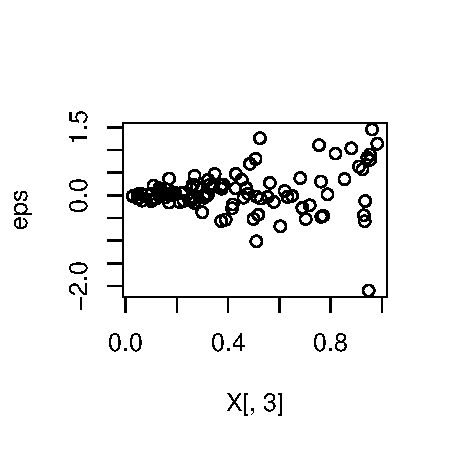
\includegraphics{figs/robust-1.pdf}

\begin{Shaded}
\begin{Highlighting}[]
\NormalTok{y <-}\StringTok{ }\NormalTok{X }\OperatorTok\StringTok{ }\NormalTok{beta }\OperatorTok{+}\StringTok{ }\NormalTok{eps}

\CommentTok{## Manual solutions}
\CommentTok{## Beta hat}
\NormalTok{beta_hat <-}\StringTok{ }\KeywordTok{solve}\NormalTok{(}\KeywordTok{t}\NormalTok{(X) }\OperatorTok\StringTok{ }\NormalTok{X, }\KeywordTok{t}\NormalTok{(X) }\OperatorTok\StringTok{ }\NormalTok{y)}
\NormalTok{beta_hat}
\end{Highlighting}
\end{Shaded}

\begin{verbatim}
##           [,1]
## [1,] 0.9503923
## [2,] 2.4367714
## [3,] 3.1610179
\end{verbatim}

Now let's get the \texttt{HC1} robust standard errors.

\begin{Shaded}
\begin{Highlighting}[]
\CommentTok{## Residuals}
\NormalTok{resid <-}\StringTok{ }\NormalTok{y }\OperatorTok{-}\StringTok{ }\NormalTok{X }\OperatorTok\StringTok{ }\NormalTok{beta_hat}
\NormalTok{sigma2_hat <-}\StringTok{ }\KeywordTok{t}\NormalTok{(resid) }\OperatorTok\StringTok{ }\NormalTok{resid }\OperatorTok{/}\StringTok{ }\NormalTok{(}\KeywordTok{nrow}\NormalTok{(X) }\OperatorTok{-}\StringTok{ }\KeywordTok{ncol}\NormalTok{(X))}
\CommentTok{## Standard, non-robust estimate}
\NormalTok{vcov_beta_hat <-}\StringTok{ }\KeywordTok{c}\NormalTok{(sigma2_hat) }\OperatorTok{*}\StringTok{ }\KeywordTok{solve}\NormalTok{(}\KeywordTok{t}\NormalTok{(X) }\OperatorTok\StringTok{ }\NormalTok{X)}
\NormalTok{vcov_beta_hat}
\end{Highlighting}
\end{Shaded}

\begin{verbatim}
##               [,1]          [,2]          [,3]
## [1,]  2.479749e-03  7.025170e-06 -0.0040547332
## [2,]  7.025170e-06  9.035269e-04 -0.0002423083
## [3,] -4.054733e-03 -2.423083e-04  0.0093815492
\end{verbatim}

\begin{Shaded}
\begin{Highlighting}[]
\CommentTok{## Robust HC1 stimate of V[\textbackslash{}hat\{\textbackslash{}bbeta\}]}
\NormalTok{vcov_rob_beta_hat <-}\StringTok{ }\KeywordTok{nrow}\NormalTok{(X)}\OperatorTok{/}\NormalTok{(}\KeywordTok{nrow}\NormalTok{(X) }\OperatorTok{-}\StringTok{ }\KeywordTok{ncol}\NormalTok{(X)) }\OperatorTok{*}\StringTok{ }
\StringTok{  }\KeywordTok{solve}\NormalTok{(}\KeywordTok{t}\NormalTok{(X) }\OperatorTok\StringTok{ }\NormalTok{X) }\OperatorTok\StringTok{ }\KeywordTok{t}\NormalTok{(X) }\OperatorTok\StringTok{ }\KeywordTok{diag}\NormalTok{(}\KeywordTok{c}\NormalTok{(resid}\OperatorTok{^}\DecValTok{2}\NormalTok{)) }\OperatorTok\StringTok{ }\NormalTok{X }\OperatorTok\StringTok{ }\KeywordTok{solve}\NormalTok{(}\KeywordTok{t}\NormalTok{(X) }\OperatorTok\StringTok{ }\NormalTok{X)}
\NormalTok{vcov_rob_beta_hat}
\end{Highlighting}
\end{Shaded}

\begin{verbatim}
##              [,1]         [,2]         [,3]
## [1,]  0.003743534  0.000355192 -0.008265779
## [2,]  0.000355192  0.003046248 -0.002539765
## [3,] -0.008265779 -0.002539765  0.022678946
\end{verbatim}

\begin{Shaded}
\begin{Highlighting}[]
\CommentTok{## Display results}
\NormalTok{outmat <-}\StringTok{ }\KeywordTok{cbind}\NormalTok{(beta_hat, }\KeywordTok{sqrt}\NormalTok{(}\KeywordTok{diag}\NormalTok{(vcov_beta_hat)),  }\KeywordTok{sqrt}\NormalTok{(}\KeywordTok{diag}\NormalTok{(vcov_rob_beta_hat)))}
\KeywordTok{colnames}\NormalTok{(outmat) <-}\StringTok{ }\KeywordTok{c}\NormalTok{(}\StringTok{"Beta Hat"}\NormalTok{, }\StringTok{"Standard SE"}\NormalTok{, }\StringTok{"HC1 Robust SE"}\NormalTok{)}
\NormalTok{outmat}
\end{Highlighting}
\end{Shaded}

\begin{verbatim}
##       Beta Hat Standard SE HC1 Robust SE
## [1,] 0.9503923  0.04979708    0.06118443
## [2,] 2.4367714  0.03005872    0.05519282
## [3,] 3.1610179  0.09685840    0.15059531
\end{verbatim}

We can do this using \texttt{lm} and the \texttt{sandwich} package.

\begin{Shaded}
\begin{Highlighting}[]
\NormalTok{lmout <-}\StringTok{ }\KeywordTok{lm}\NormalTok{(y }\OperatorTok{~}\StringTok{ }\DecValTok{0} \OperatorTok{+}\StringTok{ }\NormalTok{X)}
\KeywordTok{library}\NormalTok{(sandwich)}
\CommentTok{## HC1 Robust}
\NormalTok{vcov_rob_beta_hat <-}\StringTok{ }\KeywordTok{vcovHC}\NormalTok{(lmout, }\DataTypeTok{type =} \StringTok{"HC1"}\NormalTok{)}
\CommentTok{## HC2 Robust}
\NormalTok{vcov_robHC2_beta_hat <-}\StringTok{ }\KeywordTok{vcovHC}\NormalTok{(lmout, }\DataTypeTok{type =} \StringTok{"HC2"}\NormalTok{)}
\CommentTok{## HC3 Robust}
\NormalTok{vcov_robHC3_beta_hat <-}\StringTok{ }\KeywordTok{vcovHC}\NormalTok{(lmout, }\DataTypeTok{type =} \StringTok{"HC3"}\NormalTok{)}
\NormalTok{outmat <-}\StringTok{ }\KeywordTok{cbind}\NormalTok{(lmout}\OperatorTok{$}\NormalTok{coefficients,}
                \KeywordTok{coef}\NormalTok{(}\KeywordTok{summary}\NormalTok{(lmout))[, }\DecValTok{2}\NormalTok{],}
                \KeywordTok{sqrt}\NormalTok{(}\KeywordTok{diag}\NormalTok{(vcov_rob_beta_hat)),}
                \KeywordTok{sqrt}\NormalTok{(}\KeywordTok{diag}\NormalTok{(vcov_robHC2_beta_hat)),}
                \KeywordTok{sqrt}\NormalTok{(}\KeywordTok{diag}\NormalTok{(vcov_robHC3_beta_hat)))}
\KeywordTok{colnames}\NormalTok{(outmat) <-}\StringTok{ }\KeywordTok{c}\NormalTok{(}\StringTok{"Beta Hat"}\NormalTok{,}
                      \StringTok{"Standard SE"}\NormalTok{,}
                      \StringTok{"HC1 Robust SE"}\NormalTok{,}
                      \StringTok{"HC2 Robust SE"}\NormalTok{,}
                      \StringTok{"HC3 Robust SE"}\NormalTok{)}
\NormalTok{outmat}
\end{Highlighting}
\end{Shaded}

\begin{verbatim}
##     Beta Hat Standard SE HC1 Robust SE HC2 Robust SE HC3 Robust SE
## X1 0.9503923  0.04979708    0.06118443    0.06235143    0.06454567
## X2 2.4367714  0.03005872    0.05519282    0.05704224    0.05989300
## X3 3.1610179  0.09685840    0.15059531    0.15474172    0.16155457
\end{verbatim}

The biggest difference is between the regular standard errors and the
robust standard errors. The finite corrections are only slightly
diferent from one another.

Shameless plug: we can easily get robust standard erors using
\texttt{lm\_robust} from the
\href{https://declaredesign.org/r/estimatr/}{\texttt{estimatr}} package.

\begin{Shaded}
\begin{Highlighting}[]
\KeywordTok{library}\NormalTok{(estimatr)}
\KeywordTok{lm_robust}\NormalTok{(y }\OperatorTok{~}\StringTok{ }\DecValTok{0} \OperatorTok{+}\StringTok{ }\NormalTok{X, }\DataTypeTok{se_type =} \StringTok{"HC1"}\NormalTok{)}
\end{Highlighting}
\end{Shaded}

\begin{verbatim}
##     Estimate Std. Error  t value     Pr(>|t|)  CI Lower CI Upper DF
## X1 0.9503923 0.06118443 15.53324 4.650495e-28 0.8289582 1.071826 97
## X2 2.4367714 0.05519282 44.15015 4.952694e-66 2.3272289 2.546314 97
## X3 3.1610179 0.15059531 20.99015 7.609783e-38 2.8621279 3.459908 97
\end{verbatim}

\begin{Shaded}
\begin{Highlighting}[]
\KeywordTok{lm_robust}\NormalTok{(y }\OperatorTok{~}\StringTok{ }\DecValTok{0} \OperatorTok{+}\StringTok{ }\NormalTok{X, }\DataTypeTok{se_type =} \StringTok{"HC2"}\NormalTok{)}
\end{Highlighting}
\end{Shaded}

\begin{verbatim}
##     Estimate Std. Error  t value     Pr(>|t|) CI Lower CI Upper DF
## X1 0.9503923 0.06235143 15.24251 1.715659e-27 0.826642 1.074143 97
## X2 2.4367714 0.05704224 42.71872 1.037656e-64 2.323558 2.549984 97
## X3 3.1610179 0.15474172 20.42770 6.555414e-37 2.853898 3.468137 97
\end{verbatim}

\begin{Shaded}
\begin{Highlighting}[]
\KeywordTok{lm_robust}\NormalTok{(y }\OperatorTok{~}\StringTok{ }\DecValTok{0} \OperatorTok{+}\StringTok{ }\NormalTok{X, }\DataTypeTok{se_type =} \StringTok{"HC3"}\NormalTok{)}
\end{Highlighting}
\end{Shaded}

\begin{verbatim}
##     Estimate Std. Error  t value     Pr(>|t|)  CI Lower CI Upper DF
## X1 0.9503923 0.06454567 14.72434 1.803574e-26 0.8222871 1.078498 97
## X2 2.4367714 0.05989300 40.68541 9.181786e-63 2.3179004 2.555642 97
## X3 3.1610179 0.16155457 19.56626 1.908508e-35 2.8403768 3.481659 97
\end{verbatim}

\hypertarget{cluster-robust-estimation}{%
\section{Cluster Robust Estimation}\label{cluster-robust-estimation}}

Another problem is that your data may be clustered. You may have groups
of observations that are exposed to similar random events, or whose
responses to an event are not unrelated to the responses of others in
that group. In this case, we will assume no dependence across groups,
but estimate variance and covariance of uncertainty within gruops. For
example, imagine studying the performance of students in different
classrooms. Those in the same classroom are likely to receive similar
``shocks'' or random effects that those in other classrooms will not. We
need to account for this clustering in our data.

Again, this is not a problem for our coefficients. However, the variance
covariance matrix of the errors now has a clustered structure. Let's
imagine we have \(m\) groups, and each group has \(n_m\) observations.
Then we can write the variance covariance matrix of the errors as

\[\mathbb{E}[\bm{\epsilon}\bm{\epsilon}^\top |\mathbf{X}] = \begin{bmatrix}
\sigma_{(1,1)1}^2 & \cdots & \sigma_{(1,n_1)1}^2 & 0 & \cdots & 0 & & & & \\
\vdots &  \ddots & \vdots & \vdots & \ddots & \vdots & & & & \\
\sigma_{(n_1,1)1}^2& \cdots & \sigma_{(n_1,n_1)1}^2 & 0 & \cdots & 0 & & & & \\
0 & \cdots & 0 & \sigma_{(1,1)2}^2 & \cdots & \sigma_{(1,n_2)2}^2 & & & & \\
\vdots & \ddots & \vdots & \vdots &  \ddots & \vdots & & & & \\
0 & \cdots & 0 & \sigma_{(n_2,1)2}^2& \cdots & \sigma_{(n_2,n_2)2}^2 & & & & \\
 & & & & & & \ddots & & & \\
 & & & & & & & \sigma_{(1,1)m}^2 & \cdots & \sigma_{(1,n_m)m}^2 \\
 & & & & & & & \vdots & \ddots & \vdots\\
 & & & & & & & \sigma_{(n_m,n_m)m}^2 & \cdots & \sigma_{(n_m,n_m)m}^2
\end{bmatrix}\]

Thus we can write the variance covariance of our coefficients as
\[\mathbb{V}[\hat{\bm{\beta}}|\mathbf{X}] = (\mathbf{X}^\top \mathbf{X})^{-1} \sum^m_{g=1}\mathbf{x_g}^\top \bm{\epsilon}_g \bm{\epsilon}^\top_g \mathbf{x_g} (\mathbf{X}^\top \mathbf{X})^{-1}\]
where \(\mathbf{x_g}\) is an \(n_g \times p\) matrix of all \(p\)
covariates for the observations in group \(g\) and \(\bm{\epsilon}_g\)
is an \(n_g \times 1\) vector of errors for the \(n_g\) observations in
group \(g\). So we have this block structure where we have a full
variance covariance matrix and we need to estimate the blocks of errors.
Without getting into the derivation, we can use
\(\sum^m_{g=1} \mathbf{e}_g \mathbf{e}_g \mathbf{x_g}\mathbf{x_g}^\top\)
to estimate
\(\sum^m_{g=1} \bm{\epsilon}_g \bm{\epsilon}^\top_g \mathbf{x_g}\mathbf{x_g}^\top\).
Thus our estimated variance covariance matrix of the coefficients is
\[\widehat{\mathbb{V}[\hat{\bm{\beta}}|\mathbf{X}]}_{CR} = (\mathbf{X}^\top \mathbf{X})^{-1} \sum^m_{g=1}\mathbf{x_g}^\top \mathbf{e}_g \mathbf{e}_g \mathbf{x_g} (\mathbf{X}^\top \mathbf{X})^{-1}\]

We also apply a finite sample correction to this estimator because it is
biased in finite samples. The standard ``fancy'' corrected estimator
that Stata uses is
\[\widehat{\mathbb{V}[\hat{\bm{\beta}}|\mathbf{X}]}_{CR_{fancy}} = \frac{m}{m-1}\frac{n-1}{n-p}(\mathbf{X}^\top \mathbf{X})^{-1} \sum^m_{g=1}\mathbf{x_g}^\top \mathbf{e}_g \mathbf{e}_g \mathbf{x_g} (\mathbf{X}^\top \mathbf{X})^{-1}\]

Again, as \(m\) and \(n\) go to infinite, the correction will go to
\(1\). This should make it obvious that a small number of clusters will
require a bigger correction from the first term.

Let's do this in \texttt{R}.

\begin{Shaded}
\begin{Highlighting}[]
\CommentTok{## Generate epsilon from correlated matrix }
\CommentTok{## 10 groups, same blocks but this is not necessary}
\KeywordTok{library}\NormalTok{(clusterGeneration)}
\end{Highlighting}
\end{Shaded}

\begin{verbatim}
## Loading required package: MASS
\end{verbatim}

\begin{Shaded}
\begin{Highlighting}[]
\KeywordTok{library}\NormalTok{(mvtnorm)}
\NormalTok{block_eps <-}\StringTok{ }\KeywordTok{genPositiveDefMat}\NormalTok{(}\DecValTok{10}\NormalTok{)}
\NormalTok{sigma_eps <-}\StringTok{ }\KeywordTok{kronecker}\NormalTok{(}\KeywordTok{diag}\NormalTok{(}\DecValTok{10}\NormalTok{), block_eps}\OperatorTok{$}\NormalTok{Sigma)}
\NormalTok{eps <-}\StringTok{ }\KeywordTok{rmvnorm}\NormalTok{(}\DecValTok{1}\NormalTok{, }\DataTypeTok{mean =} \KeywordTok{rep}\NormalTok{(}\DecValTok{0}\NormalTok{, }\DecValTok{100}\NormalTok{), }\DataTypeTok{sigma =}\NormalTok{ sigma_eps}\OperatorTok{/}\DecValTok{4}\NormalTok{)}
\NormalTok{groups <-}\StringTok{ }\KeywordTok{rep}\NormalTok{(}\DecValTok{1}\OperatorTok{:}\DecValTok{10}\NormalTok{, }\DataTypeTok{each =} \DecValTok{10}\NormalTok{)}
\NormalTok{groups}
\end{Highlighting}
\end{Shaded}

\begin{verbatim}
##   [1]  1  1  1  1  1  1  1  1  1  1  2  2  2  2  2  2  2  2  2  2  3  3  3
##  [24]  3  3  3  3  3  3  3  4  4  4  4  4  4  4  4  4  4  5  5  5  5  5  5
##  [47]  5  5  5  5  6  6  6  6  6  6  6  6  6  6  7  7  7  7  7  7  7  7  7
##  [70]  7  8  8  8  8  8  8  8  8  8  8  9  9  9  9  9  9  9  9  9  9 10 10
##  [93] 10 10 10 10 10 10 10 10
\end{verbatim}

\begin{Shaded}
\begin{Highlighting}[]
\NormalTok{y <-}\StringTok{ }\NormalTok{X }\OperatorTok\StringTok{ }\NormalTok{beta }\OperatorTok{+}\StringTok{ }\KeywordTok{t}\NormalTok{(eps)}

\CommentTok{## Manual solutions}
\CommentTok{## Beta hat}
\NormalTok{beta_hat <-}\StringTok{ }\KeywordTok{solve}\NormalTok{(}\KeywordTok{t}\NormalTok{(X) }\OperatorTok\StringTok{ }\NormalTok{X, }\KeywordTok{t}\NormalTok{(X) }\OperatorTok\StringTok{ }\NormalTok{y)}
\NormalTok{beta_hat}
\end{Highlighting}
\end{Shaded}

\begin{verbatim}
##           [,1]
## [1,] 0.8392765
## [2,] 2.1686256
## [3,] 3.3014213
\end{verbatim}

\begin{Shaded}
\begin{Highlighting}[]
\CommentTok{## Residuals}
\NormalTok{resid <-}\StringTok{ }\NormalTok{y }\OperatorTok{-}\StringTok{ }\NormalTok{X }\OperatorTok\StringTok{ }\NormalTok{beta_hat}
\NormalTok{sigma2_hat <-}\StringTok{ }\DecValTok{1}\OperatorTok{/}\NormalTok{(}\KeywordTok{nrow}\NormalTok{(X) }\OperatorTok{-}\StringTok{ }\KeywordTok{ncol}\NormalTok{(X)) }\OperatorTok{*}\StringTok{ }\KeywordTok{c}\NormalTok{(}\KeywordTok{t}\NormalTok{(resid) }\OperatorTok\StringTok{ }\NormalTok{resid)}
\CommentTok{## Standard, non-robust estimate}
\NormalTok{vcov_beta_hat <-}\StringTok{ }\KeywordTok{c}\NormalTok{(sigma2_hat) }\OperatorTok{*}\StringTok{ }\KeywordTok{solve}\NormalTok{(}\KeywordTok{t}\NormalTok{(X) }\OperatorTok\StringTok{ }\NormalTok{X)}
\NormalTok{vcov_beta_hat}
\end{Highlighting}
\end{Shaded}

\begin{verbatim}
##               [,1]          [,2]         [,3]
## [1,]  0.0382446856  0.0001083478 -0.062535349
## [2,]  0.0001083478  0.0139349164 -0.003737073
## [3,] -0.0625353487 -0.0037370734  0.144689779
\end{verbatim}

\begin{Shaded}
\begin{Highlighting}[]
\CommentTok{## Cluster Robust estimate of V[\textbackslash{}hat\{\textbackslash{}bbeta\}]}
\NormalTok{meat <-}\StringTok{ }\KeywordTok{matrix}\NormalTok{(}\DecValTok{0}\NormalTok{, }\DataTypeTok{nrow =} \KeywordTok{ncol}\NormalTok{(X), }\DataTypeTok{ncol =} \KeywordTok{ncol}\NormalTok{(X))}
\ControlFlowTok{for}\NormalTok{ (g }\ControlFlowTok{in} \DecValTok{1}\OperatorTok{:}\DecValTok{10}\NormalTok{) \{}
\NormalTok{  meat <-}\StringTok{ }\NormalTok{meat }\OperatorTok{+}\StringTok{ }\KeywordTok{t}\NormalTok{(X[groups }\OperatorTok{==}\StringTok{ }\NormalTok{g, ]) }\OperatorTok\StringTok{ }\NormalTok{resid[groups }\OperatorTok{==}\StringTok{ }\NormalTok{g] }\OperatorTok
\StringTok{    }\KeywordTok{t}\NormalTok{(resid[groups }\OperatorTok{==}\StringTok{ }\NormalTok{g]) }\OperatorTok\StringTok{ }\NormalTok{X[groups }\OperatorTok{==}\StringTok{ }\NormalTok{g, ]}
\NormalTok{\}}
\NormalTok{vcov_crob_beta_hat <-}\StringTok{ }\NormalTok{(}\DecValTok{10}\OperatorTok{/}\NormalTok{(}\DecValTok{10-1}\NormalTok{)) }\OperatorTok{*}\StringTok{ }\NormalTok{((}\DecValTok{100} \OperatorTok{-}\StringTok{ }\DecValTok{1}\NormalTok{)}\OperatorTok{/}\NormalTok{(}\DecValTok{100} \OperatorTok{-}\StringTok{ }\DecValTok{3}\NormalTok{)) }\OperatorTok{*}\StringTok{ }
\StringTok{  }\KeywordTok{solve}\NormalTok{(}\KeywordTok{t}\NormalTok{(X) }\OperatorTok\StringTok{ }\NormalTok{X) }\OperatorTok\StringTok{ }\NormalTok{meat }\OperatorTok\StringTok{ }\KeywordTok{solve}\NormalTok{(}\KeywordTok{t}\NormalTok{(X) }\OperatorTok\StringTok{ }\NormalTok{X)}
\NormalTok{vcov_crob_beta_hat}
\end{Highlighting}
\end{Shaded}

\begin{verbatim}
##              [,1]         [,2]         [,3]
## [1,]  0.039699729  0.009047246 -0.058446415
## [2,]  0.009047246  0.022368271 -0.005527682
## [3,] -0.058446415 -0.005527682  0.125846996
\end{verbatim}

\begin{Shaded}
\begin{Highlighting}[]
\CommentTok{## Display results}
\NormalTok{outmat <-}\StringTok{ }\KeywordTok{cbind}\NormalTok{(beta_hat, }\KeywordTok{sqrt}\NormalTok{(}\KeywordTok{diag}\NormalTok{(vcov_beta_hat)),  }\KeywordTok{sqrt}\NormalTok{(}\KeywordTok{diag}\NormalTok{(vcov_crob_beta_hat)))}
\KeywordTok{colnames}\NormalTok{(outmat) <-}\StringTok{ }\KeywordTok{c}\NormalTok{(}\StringTok{"Beta Hat"}\NormalTok{, }\StringTok{"Standard SE"}\NormalTok{, }\StringTok{"Cluster Robust SE"}\NormalTok{)}
\NormalTok{outmat}
\end{Highlighting}
\end{Shaded}

\begin{verbatim}
##       Beta Hat Standard SE Cluster Robust SE
## [1,] 0.8392765   0.1955625         0.1992479
## [2,] 2.1686256   0.1180462         0.1495603
## [3,] 3.3014213   0.3803811         0.3547492
\end{verbatim}

\texttt{R} does not have a built in function for cluster robust standard
errors. Also, while there are scripts online to do this, estiamting
cluster robust standard errors in \texttt{estimatr} is very easy.

\begin{Shaded}
\begin{Highlighting}[]
\CommentTok{## Put data in data.frame}
\NormalTok{df <-}\StringTok{ }\KeywordTok{as.data.frame}\NormalTok{(}\KeywordTok{cbind}\NormalTok{(y, X, groups))}
\KeywordTok{names}\NormalTok{(df) <-}\StringTok{ }\KeywordTok{c}\NormalTok{(}\StringTok{"y"}\NormalTok{, }\StringTok{"x1"}\NormalTok{, }\StringTok{"x2"}\NormalTok{, }\StringTok{"x3"}\NormalTok{, }\StringTok{"groups"}\NormalTok{)}

\CommentTok{## Fit model}
\KeywordTok{library}\NormalTok{(estimatr)}
\NormalTok{lm_robustout <-}\StringTok{ }\KeywordTok{lm_robust}\NormalTok{(y }\OperatorTok{~}\StringTok{ }\NormalTok{x2 }\OperatorTok{+}\StringTok{ }\NormalTok{x3, }\DataTypeTok{data =}\NormalTok{ df, }\DataTypeTok{clusters =}\NormalTok{ groups, }\DataTypeTok{se_type =} \StringTok{"stata"}\NormalTok{)}

\CommentTok{## Display results}
\NormalTok{outmat <-}\StringTok{ }\KeywordTok{cbind}\NormalTok{(beta_hat, }\KeywordTok{sqrt}\NormalTok{(}\KeywordTok{diag}\NormalTok{(vcov_beta_hat)),  lm_robustout}\OperatorTok{$}\NormalTok{std.error)}
\KeywordTok{colnames}\NormalTok{(outmat) <-}\StringTok{ }\KeywordTok{c}\NormalTok{(}\StringTok{"Beta Hat"}\NormalTok{, }\StringTok{"Standard SE"}\NormalTok{, }\StringTok{"Cluster Robust SE"}\NormalTok{)}
\NormalTok{outmat}
\end{Highlighting}
\end{Shaded}

\begin{verbatim}
##              Beta Hat Standard SE Cluster Robust SE
## (Intercept) 0.8392765   0.1955625         0.1992479
## x2          2.1686256   0.1180462         0.1495603
## x3          3.3014213   0.3803811         0.3547492
\end{verbatim}

Same as above!

\hypertarget{some-comments}{%
\section{Some comments}\label{some-comments}}

\hypertarget{why-would-you-use-regular-standard-errors-if-heteroskedastic-standard-errors-and-clustered-standard-errors-both-allow-for-more-complicated-error-structures}{%
\subsubsection{Why would you use regular standard errors if
heteroskedastic standard errors and clustered standard errors both allow
for more complicated error
structures?}\label{why-would-you-use-regular-standard-errors-if-heteroskedastic-standard-errors-and-clustered-standard-errors-both-allow-for-more-complicated-error-structures}}

Homoskedasticity is simply a special case of the heteroskedastic error
structure; it is simply the case where \(\sigma_j = \sigma_i\) for all
\(i\) and \(j\). So using heteroskedastic standard errors will always
handle the case of homoskedasticity and will always be safe in that way.
However:

\begin{itemize}
\tightlist
\item
  Regular standard errors do not have finite sample bias. So if we truly
  believe homoskedasticity to be true, then we can avoid finite sample
  bias by using the regular standard errors.
\item
  Furthermore, if homoskedasticity actually is true, then our estimates
  of the standard errors will be more efficient. This means it will
  approach the true value faster (as the sample size grows), then
  heteroskedastic standard errors.
\item
  However, we rarely believe that errors actually are homoskedastic, and
  it is often best to use the heteroskedasticity robust standard errors
\end{itemize}

\hypertarget{remember-the-error-structure-is-not-important-for-unbiasedness-of-hatbeta-as-long-as-it-has-conditional-mean-0}{%
\subsubsection{\texorpdfstring{Remember, the error structure is not
important for unbiasedness of \(\hat{\beta}\) as long as it has
conditional mean
\(0\)}{Remember, the error structure is not important for unbiasedness of \textbackslash hat\{\textbackslash beta\} as long as it has conditional mean 0}}\label{remember-the-error-structure-is-not-important-for-unbiasedness-of-hatbeta-as-long-as-it-has-conditional-mean-0}}

Review your notes for the proof that \(\hat{\bm{\beta}}\) is an unbiased
estimator for \(\bm{\beta}\). Never do we use the variance-covariance
matrix, \(\mathbb{E}[\bm{\epsilon}\bm{\epsilon}^\top|X]\). All we use is
the conditional mean of \(\bm{\epsilon}\). This whole discussion is
about the biasedness of our estimates for
\(\mathbb{V}[\hat{\bm{\beta}}]\), which is our estimate of uncertainty
and is how we do hypothesis testing.

\hypertarget{normally-distributed-errors}{%
\subsubsection{Normally Distributed
Errors}\label{normally-distributed-errors}}

We have been very focused on the variance-covariance of
\(\bm{\epsilon}\), but not on how those errors have been distributed.
For example, it is often stated that we assume that the errors are
\textbf{normally distributed}. The normality of the errors is not
necessary for unbiasedness of either \(\hat{\bm{\beta}}\) or
\(\widehat{\mathbb{V}[\hat{\bm{\beta}}]}\). So why do people make that
assumption?

\begin{itemize}
\tightlist
\item
  Normality is somewhat important for significance testing.
  Specifically, with normal, independent standard errors we can be
  assured the \(\hat{\bm{\beta}}\) is distributed normally even in
  finite samples. This means we can get \(t\)-statistic that is actually
  \(t\)-distributed. Thus it is important for significance testing, but
  not for the standard errors themselves. Nonetheless, even without
  normal errors, \(\hat{\bm{\beta}}\) will still be distributed normally
  asymptotically, meaning as the sample size goes to \(\infty\).
  Furthermore, our test statistic will also be normally distributed and
  thus asymptotically significance testing will also be valid. These are
  the result of the central limit theorem. This generally means that if
  you have a very large sample (where ``very large'' is intentionally
  vague), then the assumption is not necessary for significance testing.
  However, in finite samples, the normality assumption guarantees that
  your confidence intervals and p-values are correct.
\item
  Normality (or perhaps other \emph{specific} distributional
  assumptions) is necessary for the ``best'' or minimum variance of the
  OLS estimator in finite samples.
\item
  Normality of the errors is needed for the standard normal linear model
  if you fit it using maximum likelihood. You will learn about this
  later in the sequence; it returns the same coefficients as OLS, but
  the framework is different. So this is largely about how you
  conceptualize regression.
\end{itemize}


\end{document}
